\section{Data} \label{sec:Data}

The empirical specification from Sect.~\ref{sec:Specification} (Eq.~\ref{eq:specification}) implies that we need data on rewards credit cards point multipliers, point values, benefits, and fees, as well as budget data for our credit card users.

\subsection{Credit Card Data}

There are many websites writing about rewards credit cards, their perks, and points structure. 
I mainly used the website allcards.com%
\footnote{\url{https://www.allcards.com} (accessed between June 3--9, 2024).}
to manually scrape the information on point multipliers and their caps (limits) from the most popular rewards credit cards from the seven major banks (American Express, Chase, Bank of America, Citi, Capital One, US Bank, and Wells Fargo). 
The bank websites were used to find some missing information, if needed. 
This resulted in a list of 27 unique credit cards.%
\footnote{Two cards, the ``Citi Double Cash'' and ``Wells Fargo Active Cash'' have identical multipliers and are included as a single card.} 
However, some of the cards have a ``custom'' bonus reward category that can be chosen by the user (e.g. 5x points on groceries, or gas, or home improvement up to \$6000 per year). 
These cards were treated as a separate credit card for each bonus category, bringing our total number of cards to 37. 

For this project I will ignore the credit cards that are dedicated to users of very specific stores, hotels, or airlines, as well as cards with rather exotic or variable reward categories (such as ``3x points on all mobile wallet payments'', or ``5x points on quarterly changing categories''), since these categories are impossible to map to our average budget that will be discussed in the next section. 
The results on total benefits should therefore be considered \emph{lower limits}, as there are many cards that can bring additional benefits to loyal users of certain brands.
In case the (prototype) model of this project is successful, I will consider adding other categories and credit cards, in combination with an online tool where a user can adjust a standard budget to his or her own spending patterns. The algorithm will then suggest the top cards to use to maximize the benefit for that specific budget. 

A list of 18 common card spending categories was taken from the website cardpointers.com,%
\footnote{\url{https://www.cardpointers.com/app/} (accessed between June 3--9, 2024).}
with the modification of removing ``warehouse clubs'' and ``ride sharing'', and adding ``streaming'' and ``travel (other)'', to facilitate a mapping of all the items on our budget to a spending category (see Sect.~\ref{subsec:UserData}). The list of categories can be found in the first column of Table~\ref{tab:BudgetExtended}.

Annual fees were also collected for all the cards in the dataset, as well as an estimate for the static benefits. If a card has a travel or food credit, this credit was taken as a benefit at full value. A \$100 ``Global Entry / TSA Precheck'' credit every five years was assumed as a \$20 yearly benefit. Airport lounge access was valued at \$40, which is approximately the value of two free meals with drinks. 

For the base and travel values of the credit card points, I used the table from the \citet{nerdwallet:2024} website. 
Finally, a boolean was added to indicate if the card is cash-back only (TRUE), or if the card allows for higher-valued travel redemptions (FALSE).
This could potentially be used to filter for certain user preferences.
All these credit card data were manually recorded in a Google Sheet and finally saved to the file \texttt{CreditCards.csv}. An exerpt of this file is shown in Fig.~\ref{fig:CreditCardsCSV}.

\subsection{User Data} \label{subsec:UserData}

For our credit card users we need a vector $\mathbf{x}$ with the amount of spend per category. The optimization algorithm will allocate the spend for each category to the credit card with the highest multiplier, turning the vector $\mathbf{x}$ into a sparse matrix $\mathbf{X}$. 
Although detailed credit card account data from real users would be very valuable for this project, regulations and privacy concerns make these data practically unavailable for researchers outside of the banking sector.  
I will therefore have to make a realistic estimate of the average spending of Americans, for which I will use the 2022 Consumer Expenditure Survey (CES) from the Bureau of Labor Statistics \citep{bls:2023}.

According to the CES, the average annual expenditures in 2022 were \$72,967 (after savings), from an average income before taxes of \$94,003.
To approximate the amount that can be spend on credit cards, I subtracted from the \$72,967 the expenses on shelter (such as mortgage, rent, property taxes), vehicle purchases, health insurance, education, cash contributions, personal insurance, and pensions.
The resulting budget totals to \$38,576 or 41 percent of the average gross income. 
The remaining CES items were then mapped to the credit card spending categories according to Table~\ref{tab:BudgetExtended}. Note that some items were split 50/50 over multiple credit card categories, to make sure that all the categories were populated with some reasonable spend. For example, I assumed that the CES item ``Apparel and services'' is split 50/50 between the ``Online shopping'' and ``Department store'' credit card categories. 

\begin{landscape}
    \begin{figure}[t!h]
        \begin{center}
        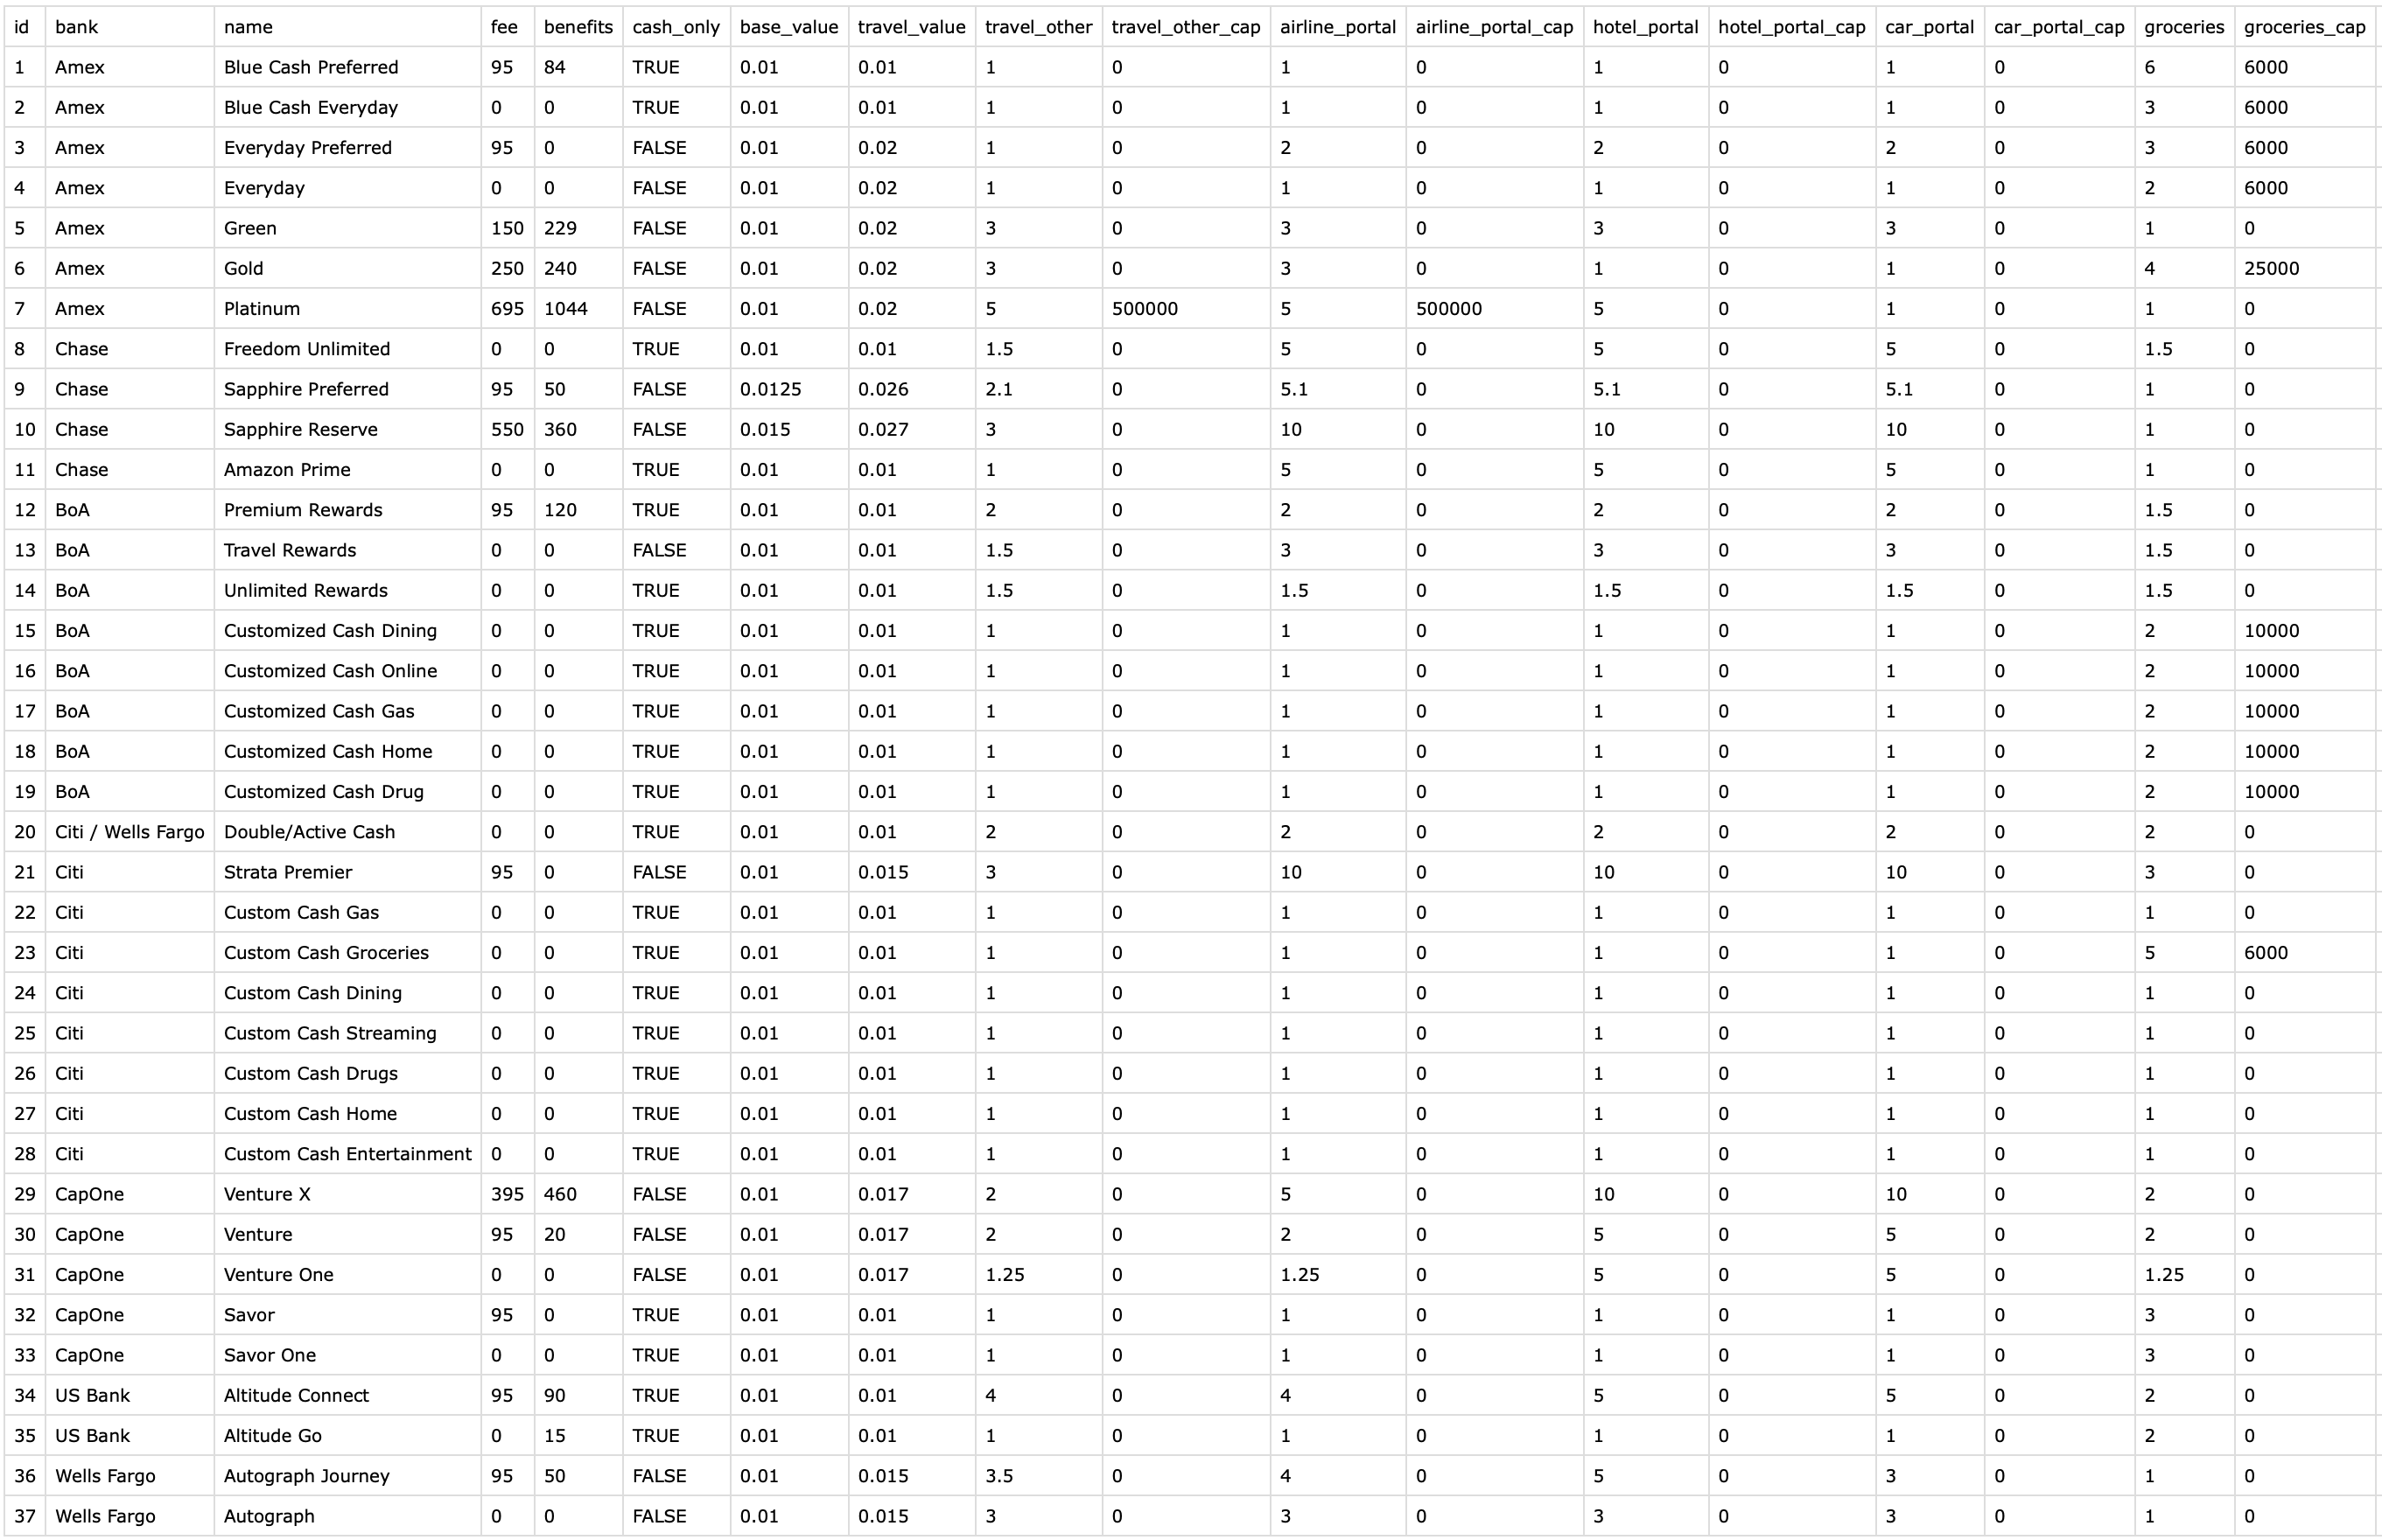
\includegraphics[scale=0.5]{../Misc/CreditCardsCSV.png}
        \caption{Exerpt of the file \texttt{CreditCards.csv} with all the 37 credit cards shown, but only 5 of the 18 categories with multipliers and their corresponding caps.}
        \label{fig:CreditCardsCSV}
        \end{center}
    \end{figure}
        
    % Table of average Credit Card Budget from the 2022 BLS Consumer Expenditure Survey    
    \begin{table}[t!bh]
    \centering
    \begin{tabular}{ r c c l} 
        \hline
        Category & Expenditure [\$] & \% & Consumer Expenditure Survey Items \\ 
        \hline
        Everything else	& 7,786 & 20.18 & Household operations, Vehicle finance charges, Maintenance and repairs, \\
        & & & Vehicle insurance, Medical services and supplies, Reading, Tobacco, Miscellaneous \\
        Groceries & 6,362 & 16.49 & Food at home, Laundry and cleaning supplies, Other household products \\
        Dining & 4,222 & 10.94 & Food away from home, Alcoholic beverages \\
        Gas	& 3,120	& 8.09 & Gasoline, other fuels, and motor oil \\
        Utility	& 3,117	& 8.08 & Utilities, fuels and public services\\
        Home improvement & 2,606 & 6.76 & Household furnishings and equipment \\
        Online shopping	& 1,881	& 4.87 & 50\% Apparel and services, Pets, toys, hobbies, and playground equipment\\
        Drug store	& 1,481 & 3.84 & Drugs, Personal care products and services \\
        Travel (other) & 1,460 & 3.78 & 50\% Other lodging, 50\% Vehicle rental, leases, licenses and other charges, \\
        & & & 50\% Public and other transportation \\
        Phone & 1,431 & 3.71 & Telephone services\\
        Streaming & 1,020 & 2.64 & Audio and visual equipment and services\\
        Department store & 973 & 2.52 & 50\% Apparel and services \\
        Entertainment & 833 & 2.16 & Fees and admissions \\
        Cable internet & 698 & 1.81 & Other entertainment supplies, equipment, and services \\
        Hotel (portal) & 644 & 1.67 & 50\% Other lodging \\
        Airline (portal) & 423 & 1.10 & 50\% Public and other transportation\\
        Car rental (portal) & 394 & 1.02 & 50\% Vehicle rental, leases, licenses and other charges \\
        Office supplies & 128 &	0.33 & Postage and stationery \\
        \hline
        \hline
        Total & 38,576	& 100.00 & \\
    \end{tabular}
    \caption{The average credit card budget as derived from the 2022 BLS Consumer Expenditure Survey. The corresponding mean income (before taxes) is \$94,003, showing that, with this budget, 41 percent of the gross income can be spend on credit cards. The first column lists the 18 credit card categories that are used throughout this project, while the last column shows how the expenditure items were mapped to each of the credit card categories.}
    \label{tab:BudgetExtended}
\end{table}


\end{landscape}

The CES also provides expenditures separated by nine income levels. 
I have repeated the above construction of the average budget also for these nine income bins separately, and saved the results in the file \texttt{BudgetIncome.csv}.
This allows for selecting the most appropriate budget as a function of the user's income (before taxes).
Our model will then predict the total credit cards benefit as a function of this income, as well as $\eta$, $\theta$, and the number of credit cards $K$ (see Sect.~\ref{sec:Specification}). 
Initially I will assume the average budget of Table~\ref{tab:BudgetExtended} (that corresponds to an average income of \$94k), as well as the budgets corresponding to an income of \$45k (low) and \$160k (high). 
For $\eta$ and $\theta$ I will assume values of 0, 0.5 and 1. 
These values can easily be adjusted, however, so I might include other values in my sensitivity analysis, in case more granularity is required. 

If successful, the prototype model will be expanded to a Monte Carlo Simulation by making many draws (with replacement) from an income distribution taken from the U.S. Census Bureau, in combination with sampling $\eta$ and $\theta$ from uniform distributions.
Such a simulation should give a reasonable estimate of the average net benefit and standard deviation for Americans who use an optimized credit card portfolio. 

% NOTES:
% Ignoring trifecta point multipliers at the moment, as well as preferred rewards value multipliers.
% Be careful not to select multiple versions of the same card when only 1 card is allowed (Citi Custom Cash).
